%% ---------------------------------------------------------------------------
%% Procedimientos para la ejecucion del proyecto.tex
%%
%% Procedimientos para la ejecucion del proyecto
%%
%% rojiark
%% ---------------------------------------------------------------------------

\chapter{Procedimientos para la ejecución del proyecto}
\label{ch:Procedimientos_para_la_ejecucion_del_proyecto}

\section{Metodología}

El proyecto primeramente consistirá en el estudio de las arquitecturas
KeyStone I y II, con el fin de establecer características propias de cada
plataforma que las diferencien tanto en su funcionamiento como en su posible
programación, incluyendo aspectos relevantes de los lenguajes que se utilizan
para programar DSP's, así como los desafíos que involucra la programación de los mismos.\\

Una vez concluido esto, se estudiará las herramientas que existen actualmente para programación en paralelo, 
con el fin de definir pruebas que puedan ser utilizadas para detectar posibles debilidades a optimizar 
dentro de las aplicaciones, en específico la existente para \newline KeyStone I.\\

Se procederá en la optimización de los puntos críticos determinados anteriormente 
y en la validación de la herramienta mediante pruebas de rendimiento, con lo cual se concluiría 
el primer objetivo específico que se plantea en este documento.\\

Se debe estudiar lo relevante a los modelos de programación en paralelo como los algoritmos
de conversión secuencial a paralelo. En específico debe dársele 
importante atención las Redes de Procesamiento de Kahn (\textit{KPNs, Kahn Process Networks}).\\

Se empezará la implementación de los algoritmos y entornos que se requieren para la generación automática
de código paralelo, así como su programación en un entorno
basado en Linux y con la herramienta de Texas Instruments Code Composer Studio (\textit{CCS}).\\

Se dispondrá a diseñar pruebas específicas para la herramienta, con el fin de 
depurar el sistema en las debilidades más notables y posteriormente comprobar la optimización de la
misma, concluyendo así el segundo objetivo específico.\\

Se pretende exponer la herramienta recién creada a un conjunto de pruebas
ya existentes y establecidas específicamente para la arquitectura KeyStone II. 
Esto con la intención de realizar un perfilado de la aplicación y determinar gráficas de rendimiento, 
realizando comparaciones entre las diferentes plataformas KeyStone y las
herramientas de generación de código.\\

Finalmente como parte integral del proyecto, se brindarán conclusiones acerca
del mismo, y los futuros proyectos que puedan involucrarse, ya sea para
optimizar la herramienta o bien en su utilización para nuevos paradigmas.

\section{Actividades a realizar durante el proyecto}

Para la finalización del primer objetivo específico se plantean las siguientes actividades
en orden cronológico:

\begin{enumerate}
 \item Estudiar las arquitecturas presentes en las tarjetas de desarrollo KeyStone I y II.
 \item Establecer diferencias importantes entre ambas tarjetas.
 \item Familiarizarse con el IDE de TI, Code Composer Studio, realizando para ello ejemplos de pruebas
 y simulaciones para tarjetas específicas.
 \item Estudiar acerca de las herramientas de Texas Instruments como el Multicore Navigator, y las
 bibliotecas \textit{IPC, Inter-Processor Communication} y \textit{openMP} .
 \item Investigar modelos de programación con estructuras en paralelo.
 \item Investigar características propias de los sistemas operativos de TI para DSP's, específicamente
 SYS/BIOS y DSP/BIOS.
 \item Estudiar a profundidad la herramienta implementada para KeyStone I para la programación
 de dispositivos de múltiples unidades de procesamiento homogéneas del tipo DSP.
 \item Realizar pruebas mediante \textit{Benchmarks} que logren poner al descubierto las debilidades
 de la herramienta.
 \item Optimizar la herramienta en los puntos más críticos que se establecieron en la actividad pasada.
 \item Comprobar la mejora o no en el rendimiento de la herramienta, utilizando como punto de partida
 la herramienta sin optimizar.\\
 
 Para cumplir con el segundo objetivo específico se proponen estas actividades: \\
 
 \item Estudiar acerca de concurrencia y paralelismo en núcleos heterogéneos
 \item Investigar sobre el funcionamiento de Colas (\textit{FIFO, First In First Out}).
 \item Estudiar a profundidad las \textit{KPNs} en donde se utilizan las \textit{FIFO}.
 \item Comprender el algoritmo que se utiliza en las \textit{KPNs} con el fin de realizar un diagrama
 de flujo del método en si.
 \item Programar el algoritmo de las \textit{KPNs} utilizando las \textit{FIFO}.
 \item Integrar el algoritmo a una herramienta que pueda ser ejecutada mediante un IDE o la línea de
 comandos de Linux.
 \item Realizar pruebas que comprueben el funcionamiento deseado de la herramienta.
 \item Determinar con el punto anterior fallos, \textit{"bugs"} y otros comportamientos no deseados 
 de la herramienta.
 \item Depurar la herramienta atacando los puntos críticos de la misma.
 \item Realizar nuevas pruebas que muestren que se ha corregido los principales fallos de la herramienta.\\
 
 Para finalizar, el tercer y último objetivo llevará acabo las siguientes actividades: \\
 
 \item Escoger algoritmos de diferente naturaleza (llámese procesamiento general, procesamiento de señales, 
 procesamiento de video e imágenes, encriptado, transmisión y comunicaciones, etc.) para ser utilizados como los
 \textit{benchmarks} de prueba de la herramienta implementada.
 \item Determinar aspectos relevantes en la ejecución de los \textit{benchmarks}, que puedan ser comparativos entre
 plataformas y herramientas.
 \item Ejecución y perfilado de las pruebas escogidas.
 \item Realización de las gráficas de rendimiento basándose en el perfilado resultante del punto anterior.
 \item Comparar las plataformas y las herramientas mediante los datos de las gráficas y del perfilado.
 \item Brindar conclusiones relevantes acerca de las pruebas realizadas
 \item Establecer recomendaciones y futuras investigaciones sobre el proyecto.
 
\end{enumerate}

\newpage
\section{Cronograma de actividades}

\begin{figure}[htb]
\centering
  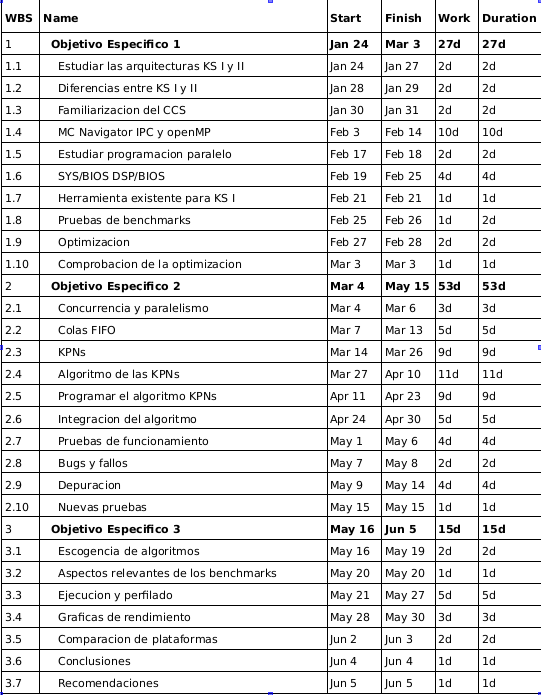
\includegraphics[width=160mm, height=175mm]{/home/rojiar/TEC/Anteproyecto/Anteproyecto/fig/Actividades.png}
  \caption{Actividades de Gantt del Proyecto de Graduación}
  \label{fig:Actividades de Gantt}
\end{figure}

\newpage

\begin{figure}[htb]
  \centering
  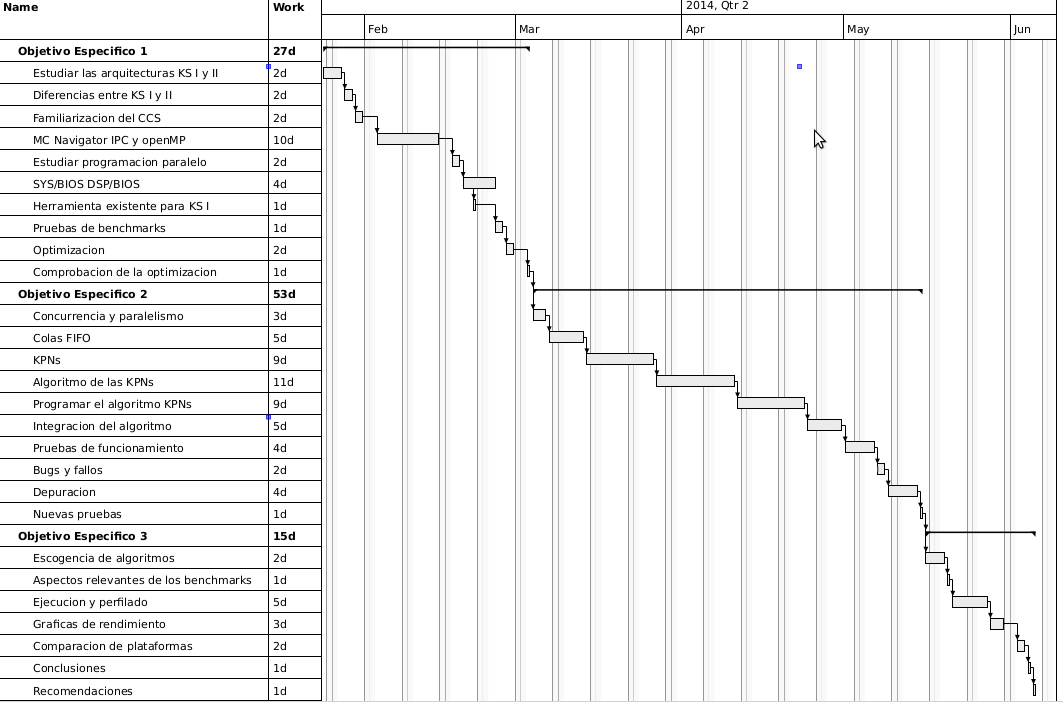
\includegraphics[width=160mm, height=150mm]{/home/rojiar/TEC/Anteproyecto/Anteproyecto/fig/diagrama.png}
  \caption{Diagrama de Gantt del Proyecto de Graduación}
  \label{fig:Diagrama de Gantt}
\end{figure}






